% Copyright (c) 2025 Carl Martin Ludvig Sinander.

% This program is free software: you can redistribute it and/or modify
% it under the terms of the GNU General Public License as published by
% the Free Software Foundation, either version 3 of the License, or
% (at your option) any later version.

% This program is distributed in the hope that it will be useful,
% but WITHOUT ANY WARRANTY; without even the implied warranty of
% MERCHANTABILITY or FITNESS FOR A PARTICULAR PURPOSE. See the
% GNU General Public License for more details.

% You should have received a copy of the GNU General Public License
% along with this program. If not, see <https://www.gnu.org/licenses/>.

%%%%%%%%%%%%%%%%%%%%%%%%%%%%%%%%%%%%%%%%%%%%%%%%%%%%%%%%%%%%%%%%%%%%%%%

In this chapter, we study the most fundamental solution concepts for normal-form games: dominance and rationalisability. These solution concepts are fundamental because they capture the implications for game play of, respectively, rationality and common knowledge of rationality. (More restrictive solutions concepts such as Nash equilibrium assume far more, viz. correct expectations of others' play.)

Throughout this chapter, we fix a finite normal-form game $\left( I, (A_i, u_i)_{i \in I} \right)$. Recall the interpretation: $I$ is a non-empty set of players, and for each player $i \in I$, $A_i$ is the non-empty set of actions available to her and $u_i : \prod_{i \in I} A_i \to \R$ is her (Bernoulli) payoff function. What it means for the game to be `finite' is that both the set $I$ of players and the action sets $A_i$ (for each player $i \in I$) are finite. It is important to remember that the ingredients $\left( I, (A_i, u_i)_{i \in I} \right)$ are always assumed to be commonly known among the players.

As usual, we write $(a_i)_{i \in I} = a \in A \coloneqq \prod_{i \in I} A_i$ for action profiles, write $a_{-j} = (a_i)_{i \in I \setminus \{j\}} \in \prod_{i \in I \setminus \{j\}} A_i \eqqcolon A_{-j}$ for profiles of actions of all players but $j \in I$, and interpret $(a_j,a_{-j}) \equiv a \in A \equiv A_j \times A_{-j}$ for each player $j \in I$.%
	\footnote{See \cref{math:set} for a review of (Cartesian) product sets.}

A \emph{mixed action} of player $i \in I$ is a probability distribution $\alpha_i \in \Delta(A_i)$ over $i$'s actions. A \emph{mixed action profile} is a (joint) probability distribution $\alpha \in \Delta(A)$ over action profiles, and a mixed action profile of all players but $j \in I$ is a (joint) probability distribution $\alpha_{-j} \in \Delta(A_{-j})$. Note that these definitions do \emph{not} assume that players mix independently. When independent mixing is intended, we indicate this by considering a \emph{profile of mixed actions,} $(\alpha_i)_{i \in I} \in \prod_{i \in I} \Delta(A_i)$ or $(\alpha_i)_{i \in I \setminus \{j\}} \in \prod_{i \in I \setminus \{j\}} \Delta(A_i)$.

Each pure action profile $a \in A$ may be identified with a degenerate mixed action profile, viz. the $\alpha \in \Delta(A)$ that is degenerate at $a$ (explicitly, $\alpha(a)=1$ and $\alpha(b)=0$ for every $b \in A \setminus \{a\}$). In this way, we may view $A$ as a subset of $\Delta(A)$ (formally, we identify $A$ with the vertices of the simplex $\Delta(A)$).

It is convenient to extend each player~$i$'s payoff function $u_i : A \to \R$ linearly to $\Delta(A)$. That is, we write $u_i(\alpha)$ for player~$i$'s \emph{expected} payoff from mixed action profile $\alpha \in \Delta(A)$: explicitly, $u_i(\alpha) \coloneqq \sum_{a \in A} u_i(a) \alpha(a)$.



%%%%%%%%%%%%%%%%%%%%%%%%%%%%%%%%%%%
%%%%%%%%%%%%%%%%%%%%%%%%%%%%%%%%%%%
\section{Best replies}
\label{dom:br}
%%%%%%%%%%%%%%%%%%%%%%%%%%%%%%%%%%%
%%%%%%%%%%%%%%%%%%%%%%%%%%%%%%%%%%%

In problems of choice under uncertainty, (Bayesian) rationality means choosing so as to maximise one's expected payoff, where the expectation is with respect to \emph{some} (subjective) belief. In this section, we explore the implications of rationality for play.

In a normal-form game, the (only) uncertainty facing a player $i \in I$ is what actions $a_{-i} \in A_{-i}$ the other players will choose. Rationality thus means choosing an action $a_i \in A_i$ which is expected-payoff maximising given some belief $\alpha_{-i} \in \Delta(A_{-i})$ about this uncertainty. We shall call such a belief $\alpha_{-i}$ a \emph{conjecture (about opponents' play).}

Note that we do not require $i$ to believe that the other players' actions are statistically independent of each other. Allowing rational players to have such `correlated' beliefs $\alpha_{-i}$ is reasonable in most applications of game theory, where the normal-form game is not literally an exhaustive description of an economic environment, but rather a metaphor capturing the essence of a strategic interaction, embedded in a larger reality that may well feature opportunities for players to correlate their actions, for example by choosing based on publicly observable events (`sunspots') such as the contents of the newspaper, the weather etc.

However, if we \emph{do} take the normal-form game literally as an exhaustive description of the strategic interaction, then a player~$i$'s understanding of the game itself entails recognising that it is simply impossible for her opponents to correlate their actions, in which case rationality demands in addition that $i$'s conjecture $\alpha_{-i} \in \Delta(A_{-i})$ be the product of its marginals (exhibiting statistical independence), i.e. $\alpha_{-i}((a_j)_{j \in I \setminus \{i\}}) = \prod_{j \in I \setminus \{i\}} \alpha_j(a_j)$ for all pure action profiles $(a_j)_{j \in I \setminus \{i\}} \in A_{-i}$.

We shall privilege the former case, allowing for `correlated' conjectures $\alpha_{-i}$ in most of this chapter. Toward the end of the chapter (\cref{dom:indp}), we consider the latter case, asking in particular how our analysis changes if players believe that their opponents' actions are statistically independent of each other. (Of course the distinction between the cases collapses when there are only two players, since then each player~$i$ has only one opponent.)

\begin{definition}
	%
	\label{definition:br}
	%
	An action $a_i \in A_i$ of player $i \in I$ is a \emph{best reply} to conjecture $\alpha_{-i} \in \Delta(A_{-i})$ iff $u_i(a_i,\alpha_{-i}) \geq u_i(b_i,\alpha_{-i})$ for every action $b_i \in A_i$.
	%
\end{definition}

More generally, a mixed action $\alpha_i \in \Delta(A_i)$ of player $i \in I$ is a best reply to conjecture $\alpha_{-i} \in \Delta(A_{-i})$ iff it assigns strictly positive probability only to (pure) best replies $a_i \in A_i$; equivalently, iff $u_i(\alpha_i,\alpha_{-i}) \geq u_i(b_i,\alpha_{-i})$ for every action $b_i \in A_i$.

% It is sometimes useful to speak more generally of \emph{better replies.} For pure actions $a_i,b_i \in A_i$ of a player $i \in I$ and a conjecture $\alpha_{-i} \in \Delta(A_{-i})$, we say that $a_i$ is a \emph{better reply (to $\alpha_{-i}$) than} $b_i$ iff $u_i(a_i,\alpha_{-i}) \geq u_i(a_i,\alpha_{-i})$. By inspection, an action is a best reply (to $\alpha_{-i}$) iff it is a better reply (to $\alpha_{-i}$) than every (other) action.

\begin{definition}
	%
	\label{definition:sbr}
	%
	An action $a_i \in A_i$ of player $i \in I$ is \emph{sometimes-best} iff there exists a conjecture $\alpha_{-i} \in \Delta(A_{-i})$ such that $a_i$ is a best reply to $\alpha_{-i}$. An action that is not sometimes-best is called \emph{never-best.}%
		\footnote{One could extend the definition of sometimes-best and never-best to mixed actions $\alpha_i \in \Delta(A_i)$ in the obvious way, but that is typically not done.}
	%
\end{definition}

Evidently if a player is (Bayesian) rational and understands the game, then she must play a sometimes-best action (equivalently, \emph{not} play a never-best action). Conversely, \emph{every} sometimes-best action is consistent with (Bayesian) rationality and comprehension of the game: if we observe a player choosing a sometimes-best action, we cannot conclude that she is irrational or fails to understand the game. In short, `play a sometimes-best action' (equivalently, `avoid never-best actions') fully characterises the implications for play of rationality and comprehension of the game.

\begin{example}
	%
	\label{example:rbty_neverbest}
	%
	Consider the following normal-form game with players $I = \{1,2\}$, in which player~1 chooses which row ($A_1 = \{U,D\}$) and player~2 chooses which column ($A_2 = \{L,M,R\}$), and as usual player~1's payoff is listed first and $2$'s second:
	%
	\begin{equation*}
		\begin{array}{c|ccc}
			  & L   & M   & R \\ \hline
			U & 0,0 & 1,1 & 0,3 \\
			D & 1,3 & 0,1 & 1,0
		\end{array}
	\end{equation*}
	%
	Both of player~1's actions are sometimes-best: for example, $U$ is a best reply to the (pure) conjecture $M$, and $D$ is a best reply to $L$. Player~2's actions $L$ and $R$ are also sometimes-best ($L$ is a best reply to $D$, and $R$ is a best reply to $U$). But player~2's action $M$ is never-best: for any conjecture of player~2 about player~1's behaviour, letting $p \in [0,1]$ denote the (conjectured) probability that $U$ is played, player~2's payoffs from her three actions $L$, $M$ and $R$ are, respectively, $3(1-p)$, $1$ and $3p$, drawn in \Cref{fig:neverbest}.
	%
	\begin{figure}
		\centering
		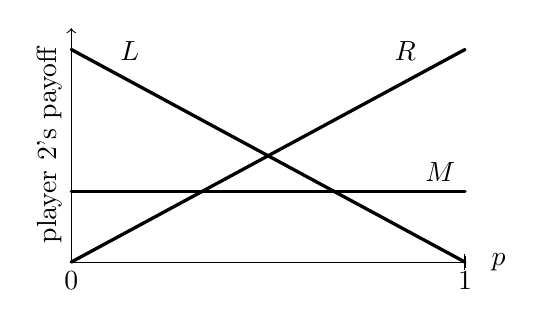
\begin{tikzpicture}[scale=1, line cap=round]

			% constants
			\pgfmathsetmacro{\xmax}{5};
			\pgfmathsetmacro{\ymax}{3};
			\pgfmathsetmacro{\ticklength}{1/14};
			\pgfmathsetmacro{\yscale}{0.9};
			\pgfmathsetmacro{\labelshift}{0.9};

			% x axis
			\draw[-|] (0,0) -- ( \xmax, 0.0 );
			\draw ( {\xmax+3*\ticklength}, 0.0 )
				node[anchor=west] {$p$};
			\draw[-] ( \xmax, - \ticklength )
				-- ( \xmax, \ticklength );
			\draw ( 0, 0.0 )
				node[anchor=north] {$0$};
			\draw ( \xmax, 0.0 )
				node[anchor=north] {$1$};

			% x axis
			\draw[->] (0,0) -- ( 0.0, {\yscale*1.1*\ymax} );
			\draw ( 0.0, {(\yscale*1.1*\ymax)/2} )
				node[anchor=east] {\rotatebox{90}{player~2's payoff}};

			% payoffs
			\draw[-,very thick] (0,0)
				-- ( \xmax, {\yscale*\ymax} );
			\draw[-,very thick] ( 0, { \yscale*\ymax} )
				-- ( \xmax, 0 );
			\draw[-,very thick] ( 0, {\yscale*\ymax/3} )
				-- ( \xmax, {\yscale*\ymax/3} );

			\draw ( {\labelshift*\xmax}, {\yscale*\labelshift*\ymax} )
				node[anchor=south east] {$R$};
			\draw ( {(1-\labelshift)*\xmax}, {\yscale*\labelshift*\ymax} )
				node[anchor=south west] {$L$};
			\draw ( \xmax, {\yscale*\ymax/3} )
				node[anchor=south east] {$M$};

		\end{tikzpicture}
		\caption{Player~2's action payoffs in \Cref{example:rbty_neverbest} as a function of the probability $p$ that player~1 plays $U$.}
		\label{fig:neverbest}
	\end{figure}
	%
	There is no $p \in [0,1]$ for which $M$ is weakly best, so $M$ is a never-best action.
	%
\end{example}

In the next section, we characterise rational play (i.e. sometimes-best actions) in terms of a seemingly different solution concept: strict dominance.



%%%%%%%%%%%%%%%%%%%%%%%%%%%%%%%%%%%
%%%%%%%%%%%%%%%%%%%%%%%%%%%%%%%%%%%
\section{Dominance}
\label{dom:dom}
%%%%%%%%%%%%%%%%%%%%%%%%%%%%%%%%%%%
%%%%%%%%%%%%%%%%%%%%%%%%%%%%%%%%%%%

\begin{definition}
	%
	\label{definition:dominates}
	%
	For mixed actions $\alpha_i,\beta_i \in \Delta(A_i)$ of a player $i \in I$, we say that $\alpha_i$ \emph{strictly dominates} $\beta_i$ iff $u_i(\alpha_i,a_{-i}) > u_i(\beta_i,a_{-i})$ for every (pure) profile $a_{-i} \in A_{-i}$ of other players' actions.
	%
\end{definition}

This definition covers strict dominance by/of pure actions, too, since pure actions $a_i,b_i \in A_i$ are a special case of mixed actions $\alpha_i,\beta_i \in \Delta(A_i)$ (namely, degenerate mixed actions).

\begin{example}
	%
	\label{example:prisoners}
	%
	Consider the prisoner's dilemma: players $I=\{1,2\}$, actions $A_1=A_2=\{C,D\}$ and payoffs
	%
	\begin{equation*}
		\begin{array}{c|ccc}
			  & C   & D   \\ \hline
			C & 2,2 & 0,3 \\
			D & 3,0 & 1,1
		\end{array}
	\end{equation*}
	%
	For both players, the action $C$ is strictly dominated by the (pure) action $D$.
	%
\end{example}

The fact that the definition quantifies only over pure profiles $a_{-i} \in A_{-i}$ does not matter: the alternative definition that quantifies over all mixed action profiles $\alpha_{-i} \in \Delta(A_{-i})$ is in fact equivalent.

\begin{exercise}[easy]
	%
	\label{exercise:dominates_others_mixed}
	%
	Prove it! That is, prove that for mixed actions $\alpha_i,\beta_i \in \Delta(A_i)$ of a player $i \in I$, $u_i(\alpha_i,a_{-i}) > u_i(\beta_i,a_{-i})$ for every pure profile $a_{-i} \in A_{-i}$ if and only if $u_i(\alpha_i,\alpha_{-i}) > u_i(\beta_i,\alpha_{-i})$ for every mixed profile $\alpha_{-i} \in \Delta(A_{-i})$.
	%
\end{exercise}

\begin{definition}
	%
	\label{definition:dominated}
	%
	A (pure) action $a_i \in A_i$ of player $i \in I$ is called \emph{strictly dominated} iff there is a mixed action $\beta_i \in \Delta(A_i)$ that strictly dominates $a_i$.%
		\footnote{One could extend the definition of `strictly dominated' to mixed actions $\alpha_i \in \Delta(A_i)$ in the obvious way, but that is typically not done.}
	%
\end{definition}

The fact that we contemplate strict domination by a \emph{mixed} action $\beta_i \in \Delta(A_i)$ matters: an action can easily be strictly dominated without being strictly dominated by a pure action.

\addtocounter{example}{-2}
\begin{example}[continued from \cpageref{example:rbty_neverbest}]
	%
	\label{example:rbty_neverbest_dom}
	%
	No pure action strictly dominates $M$:
	$M$ is better than $L$ against $U$, and better than $R$ against $D$. But $M$ is strictly dominated by a mixed action, namely the $50$--$50$ mix of $L$ and $R$: this mixed action yields an expected payoff of $1.5$ regardless of player~1's choice, strictly better than action $M$'s payoff of $1$.
	%
\end{example}
\addtocounter{example}{1}

% \begin{definition}
% 	%
% 	\label{definition:dominant}
% 	%
% 	A (pure) action $a_i \in A_i$ of player $i \in I$ is called \emph{strictly dominant} iff it strictly dominates every other (pure) action $b_i \in A_i \setminus \{a_i\}$.%
% 		\footnote{It makes no difference if we instead require $a_i$ to strictly dominate every other \emph{mixed} action $\beta_i \in \Delta(A_i) \setminus \{a_i\}$. Nor do we need to consider the possibility of a strictly dominant mixed action $\alpha_i \in A_i$, since an implication of such a definition would be that a strictly dominant action must be pure (why?).}
% 	%
% \end{definition}

Recall from the previous section that (Bayesian) rationality plus comprehension of the game entails nothing more or less than that no player plays a never-best action. The following shows that this is equivalent to eschewing strictly dominated actions.

\begin{namedthm}[Pearce's lemma.]
	%
	\label{lemma:pearce}
	%
	An action of a player is never-best if and only if it is strictly dominated.
	%
\end{namedthm}

\addtocounter{example}{-2}
\begin{example}[continued]
	%
	\label{example:rbty_neverbest_pearce}
	%
	We saw that player~2's action $M$ is never-best, and that it is strictly dominated. We also saw that player~2's other actions, $L$ and $R$, are sometimes-best (not never-best), and it may be verified that they are not strictly dominated. Similarly for both of player~1's actions, $U$ and $D$.
	%
\end{example}
\addtocounter{example}{1}

The proof relies on the separating hyperplane theorem.%
	\footnote{See e.g. Theorem~M.G.2 in \textcite[][p.~948]{MascolellWhinstonGreen1995}. For a fuller treatment, consider \textcite{Border2016}.}

\begin{proof}
	%
	For the `if' direction, suppose that $a_i$ is strictly dominated: there is a mixed action $\beta_i \in \Delta(A_i)$ such that $u_i(a_i,a_{-i}) < u_i(\beta_i,a_{-i})$ for all (pure) profiles $a_{-i} \in A_{-i}$. Then $u_i(a_i,\alpha_{-i}) < u_i(\beta_i,\alpha_{-i})$ for any conjecture $\alpha_{-i} \in \Delta(A_{-i})$, so $a_i$ is never-best.

	For the `only if' direction, we prove the contra-positive: we assume that $a_i$ is \emph{not} strictly dominated, and establish the existence of a conjecture $\alpha_{-i} \in \Delta(A_{-i})$ to which $a_i$ is a best reply (hence $a_i$ is not never-best). Enumerate the other players' action profiles $A_{-i}$ (a finite set) as $A_{-i} \equiv \{1,\dots,N\}$ where $N \coloneqq \abs*{A_{-i}}$. For each mixed action $\alpha_i \in \Delta(A_i)$, let $U^{\alpha_i} \in \R^N$ be the vector 
	%
	\begin{equation*}
		U^{\alpha_i} \coloneqq \bigl( u_i(\alpha_i,1), u_i(\alpha_i,2), \dots, u_i(\alpha_i,N) \bigr) ,
	\end{equation*}
	%
	and let
	%
	\begin{equation*}
		\mathcal{U} \coloneqq \left\{ v \in \R^N : \text{$v = U^{a_i} - U^{\alpha_i}$ for some $\alpha_i \in \Delta(A_i)$} \right\} .
	\end{equation*}
	%
	Observe that $\mathcal{U}$ is a convex subset of $\R^N$, and that $\boldsymbol{0} \coloneqq (0,0,\dots,0)$ is a member.%
		\footnote{For any $v,w \in \mathcal{U}$, we have $v = U^{a_i} - U^{\alpha_i}$ and $w = U^{a_i} - U^{\beta_i}$ for some $\alpha_i,\beta_i \in \Delta(A_i)$, which since $u_i(\cdot,n)$ is linear for each $n \in \{1,\dots,N\}$ implies that for any $\lambda \in (0,1)$, $\lambda v + (1-\lambda) w = U^{a_i} - U^{\lambda \alpha_i + (1-\lambda) \beta_i} \in \mathcal{U}$.}
	Since (by hypothesis) $a_i$ is not strictly dominated, it holds that for each $\alpha_i \in \Delta(A_i)$, there is an $n \in \{1,\dots,N\}$ such that $u_i(a_i,n) \geq u_i(\alpha_i,n)$; in other words, the $n$th entry of $U^{a_i}-U^{\alpha_i}$ is non-negative. Hence every element of $\mathcal{U}$ has at least one non-negative entry, which is to say that $\mathcal{U}$ is disjoint from the negative orthant
	%
	\begin{equation*}
		\R_{--}^N \coloneqq \{ v \in \R^N : \text{$v_n < 0$ for every $n \in \{1,\dots,N\}$} \} .
	\end{equation*}

	Since both $\mathcal{U}$ and $\R_{--}^N$ are convex, it follows by the separating hyperplane theorem that there exists a vector $v \in \R^N \setminus \{\boldsymbol{0}\}$ and a constant $c \in \R$ such that $u \cdot v \geq c$ for every $u \in \mathcal{U}$ and $u \cdot v \leq c$ for every $u \in \R_{--}^N$. It must be that $c=0$, since $\boldsymbol{0}$ belongs both to $\mathcal{U}$ and to the closure of $\R_{--}^N$.%
		\footnote{On the one hand, $c \leq \boldsymbol{0} \cdot v = 0$ since $u \in \mathcal{U}$. On the other hand, we have $c \geq (-\varepsilon,\dots,-\varepsilon) \cdot v$ for every $\varepsilon>0$ since $(-\varepsilon,\dots,-\varepsilon) \in \R_{--}^N$, so letting $\varepsilon \downarrow 0$ yields $c \geq \boldsymbol{0} \cdot v = 0$.}
	Furthermore, $v$ must have only non-negative entries, since otherwise we could find a $u \in \R_{--}^N$ such that $u \cdot v > 0$.%
		\footnote{If $v_n < 0$ for some $n \in \{1,\dots,N\}$, then $u \cdot v > 0$ for the vector $u \in \R_{--}^N$ defined by $u_n \coloneqq - 2 ( 1 + \sum_{m \neq n} \abs*{v_m} ) / (-v_n)$ and $u_m \coloneqq -1$ for each $m \in \{1,\dots,N\} \setminus \{n\}$.}
	Define
	%
	\begin{equation*}
		\alpha_{-i} \coloneqq \frac{v}{ \sum_{n=1}^N v_n } \in \Delta(A_{-i}) .
	\end{equation*}
	%
	The action $a_i$ is a best reply to the conjecture $\alpha_{-i}$, since for any other action $b_i \in A_i$, 
	%
	\begin{align*}
		u_i(a_i,\alpha_{-i})
		- u_i(b_i,\alpha_{-i})
		&= \sum_{n=1}^N
		\left[ u_i(a_i,n) - u_i(b_i,n) \right]
		\left[\alpha_{-i}\right]_n
		\\
		&= \left( U^{a_i} - U^{b_i} \right)
		\cdot \alpha_{-i}
		\geq 0 .
		\qedhere
	\end{align*}
	%
\end{proof}

\begin{remark}
	%
	\label{remark:pearce_finite}
	%
	The above proof relies on the assumption, maintained throughout this chapter, that the game under consideration is finite. 
	The `only if' part of \hyperref[lemma:pearce]{Pearce's lemma} is not generally true for non-finite games, as shown in \Cref{exercise:pearce_counterex} below. (The `if' part \emph{is} generally true.)
	It turns out, however, that the finiteness assumption in \hyperref[lemma:pearce]{Pearce's lemma} can be substituted with compactness of action sets and (upper semi-)continuity of payoffs.
	%
\end{remark}

\begin{exercise}
	%
	\label{exercise:pearce_counterex}
	%
	Consider the normal-form game $\left(I,(A_i,u_i)_{i \in I}\right)$ where $I = \{1,2\}$, $A_1 \coloneqq [0,1]$ and $A_2 = [0,1)$, and $u_1(a_1,a_2) \coloneqq - (a_1-a_2)^2$ for all $a_1 \in A_1$ and $a_2 \in A_2$.

	\begin{enumerate}[label=(\alph*)]
	
		\item Prove that player~1's action $a_1 = 1$ is never-best.

		\item Prove that player~1's action $a_1 = 1$ is \emph{not} strictly dominated. (Not even weakly dominated, in fact.)
	
	\end{enumerate}
	%
\end{exercise}



%%%%%%%%%%%%%%%%%%%%%%%%%%%%%%%%%%%
%%%%%%%%%%%%%%%%%%%%%%%%%%%%%%%%%%%
\section{Rationalisability}
\label{dom:rbty}
%%%%%%%%%%%%%%%%%%%%%%%%%%%%%%%%%%%
%%%%%%%%%%%%%%%%%%%%%%%%%%%%%%%%%%%

We have seen that the (only) implication of rationality and comprehension of the game is that players will not choose never-best (equivalently, strictly dominated) actions. But what if each player additionally knows that her opponents are rational?

\addtocounter{example}{-2}
\begin{example}[continued from \cpageref{example:rbty_neverbest,example:rbty_neverbest_dom,example:rbty_neverbest_pearce}]
	%
	\label{example:rbty_neverbest_rbty}
	%
	If player~2 is rational, then she will not play the never-best action $M$. Hence if player~1 knows that player~2 is rational, then she can rule out the possibility that player~2 will play $M$. Once the possibility of $M$ has been ruled out, rationality requires player~1 to choose action $D$, since it is strictly better than $U$ (payoff $1>0$) against player~2's remaining actions $\{L,R\}$. To summarise, rationality does \emph{not} require player~1 to chose $D$ (her other action $U$ is not never-best), but rationality plus knowledge of player~2's rationality does require player~1 to choose $D$.
	%
\end{example}
\addtocounter{example}{1}

Going further, it may be that each player $i \in I$ knows not only that players $j \in I \setminus \{i\}$ are rational, but also that players $j \in I \setminus \{i\}$ know that all players $k \in I \setminus \{j\}$ are rational.

\addtocounter{example}{-2}
\begin{example}[continued]
	%
	\label{example:rbty_neverbest_rbty1}
	%
	We saw that if player~1 is rational and knows that player~2 is rational, then she must play $D$. If in addition player~2 knows that player~1 knows than player~2 is rational, then player~2 understands that player~1 must play $D$. So if in addition player~2 is herself rational, she must play a best reply to $D$: in other words, she must play $L$. Thus rationality, knowledge of rationality and knowledge of knowledge of rationality together yield a unique prediction of play in this game.
	%
\end{example}
\addtocounter{example}{1}

Further still, it may be that for all players $i,j,k,\ell \in I$ such that $i \neq j \neq k \neq \ell$, player~$i$ knows not only that player~$j$ is rational and that player~$j$ knows that player~$k$ is rational, but also that player~$j$ knows that player~$k$ knows that player~$\ell$ is rational. And so on.

If all statements of the above form are true, we say that it is \emph{commonly known} that all players are rational; more concisely, there is `common knowledge of rationality'. The implications for play of rationality (of all players) and common knowledge (among all players) of rationality are precisely captured by \emph{rationalisability.}

\begin{definition}
	%
	\label{definition:rbty}
	%
	For each player $i \in I$ and each conjecture $\alpha_{-i} \in \Delta(A_{-i})$, write $\text{BR}_i(\alpha_{-i}) \subseteq A_i$ for the set of best replies to $\alpha_{-i}$.
	Define $X^0_i \coloneqq A_i$ and $X^0_{-i} \coloneqq A_{-i}$ for each $i \in I$.
	For each $t \in \N$, iteratively define
	%
	\begin{equation*}
		X^t_i \coloneqq \text{BR}_i\left( \Delta\left( X^{t-1}_{-i} \right) \right)
		\equiv \Union_{\alpha_{-i} \in \Delta\left( X^{t-1}_{-i} \right)} \text{BR}_i(\alpha_{-i})
		\quad \text{for each $i \in I$,}
	\end{equation*}
	%
	$X^t_{-j} \coloneqq \prod_{i \in I \setminus \{j\}} X^t_i$ for each $j \in I$, and $X^t \coloneqq \prod_{i \in I} X^t_i$.
	Finally, define $X^\infty_i \coloneqq \Intersect_{t \in \N} X^t_i$ for each $i \in I$, and $X^\infty \coloneqq \prod_{i \in I} X^\infty_i$. An action $a_i \in A_i$ of player $i \in I$ is called \emph{rationalisable} iff it belongs to $X^\infty_i$; similarly, an action profile $a = (a_i)_{i \in I} \in A$ is called rationalisable iff it belongs to $X^\infty$.
	%
\end{definition}

The procedure (or algorithm) described in \Cref{definition:rbty} is called \emph{iterated deletion of never-best actions.} By \hyperref[lemma:pearce]{Pearce's lemma}, it is equivalent to the more familiar procedure of \emph{iterated deletion of strictly dominated actions,} provided (crucially) that in each round, remaining actions that are strictly dominated by a remaining \emph{mixed} action are deleted.

\addtocounter{example}{-2}
\begin{example}[continued]
	%
	\label{example:rbty_neverbest_rbty2}
	%
	In the language of iterated deletion, our previous reasoning may be summarised as
	%
	\begin{align*}
		X^1 &= X^1_1 \times X^1_2 = \{U,D\} \times \{L,R\} ,
		\\
		X^2 &= X^2_1 \times X^2_2 = \{D\} \times \{L,R\} ,
		\\
		X^3 &= X^3_1 \times X^3_2 = \{D\} \times \{L\} ,
	\end{align*}
	%
	and $X^\infty = X^t = X^3$ for all $t \geq 4$. In particular, $D$ ($L$) is the unique rationalisable action of player~1 (player~2).
	%
\end{example}
\addtocounter{example}{1}

In the example, for each player $i \in I$, the sets $(X^t_i)_{t \in \N}$ are nested in the sense that $X^{t-1}_i \supseteq X^t_i$ for each $t \in \N$, and the set $X^\infty_i$ of rationalisable actions is non-empty. These features are general:

\begin{proposition}
	%
	\label{proposition:rbty_nonempty}
	%
	For each player $i \in I$, $X^{t-1}_i \supseteq X^t_i$ for each $t \in \N$, and the set $X^\infty_i$ of rationalisable actions is non-empty.
	%
\end{proposition}

This is a reassuring result, since if there were no rationalisable actions then we would be faced with the paradox that the game itself is somehow inconsistent with rationality and common knowledge of rationality!

\begin{proof}
	%
	We prove the first (nestedness) claim by induction on $t \in \N$.%
		\footnote{See \cref{math:pf} for a review of mathematical induction.}
	The base case $t=1$ is immediate: $X^0_i = A_i \supseteq X^1_i$ for every $i \in I$. For the induction step, fix any $t \in \N$, and suppose that $X^{t-1}_i \supseteq X^t_i$ for every player $i \in I$; we will show that $X^t_i \supseteq X^{t+1}_i$ for every player $i \in I$. So fix any player $i \in I$. Since $X^{t-1}_{-i} \supseteq X^t_{-i}$ (by the induction hypothesis), we have $\Delta(X^{t-1}_{-i}) \supseteq \Delta(X^t_{-i})$, and thus
	%
	\begin{equation*}
		X^t_i
		= \Union_{\alpha_{-i} \in \Delta(X^{t-1}_{-i})} \text{BR}_i(\alpha_{-i})
		\supseteq \Union_{\alpha_{-i} \in \Delta(X^t_{-i})} \text{BR}_i(\alpha_{-i})
		= X^{t+1}_i .
	\end{equation*}

	Toward proving the second (non-emptiness) claim, we first show that $X^t_i$ is non-empty for each $i \in I$ and $t \in \N$. We again employ induction on $t \in \{0,1,2,\dots\}$. For the base case $t=0$, obviously $X^0_i = A_i$ is non-empty for every $i \in I$. For the induction step, suppose for some $t \in \N$ that $X^{t-1}_i$ is non-empty for every $i \in I$; we will show that $X^t_i$ is also non-empty for every $i \in I$. To that end, fix any player $i \in I$ and an arbitrary element $\alpha_{-i}$ of the (by the induction hypothesis) non-empty set $\Delta(X^{t-1}_{-i})$. Since $A_i$ is (non-empty and) finite, there must be a best reply of player~$i$ to $\alpha_{-i}$. By definition, this best-reply action belongs to $X^t_i$; so $X^t_i$ is non-empty.

	We have shown that for each player $i \in I$, $A_i \supseteq X^{t-1}_i \supseteq X^t_i \neq \varnothing$ for every $t \in \N$. Since $A_i$ is finite for every player $i \in I$, it follows that the iteration must eventually terminate: $X^{T-1} = X^T \neq \varnothing$ for some $T \in \N$, so $X^t = X^{T-1}$ for all $t \geq T$. Then $X^\infty = X^{T-1} \neq \varnothing$.
	%
\end{proof}

\begin{remark}
	%
	\label{remark:rbty_nonempty_finite}
	%
	The above proof relies on the assumption, maintained throughout this chapter, that the game under consideration is finite.
	Like \hyperref[lemma:pearce]{Pearce's lemma}, \Cref{proposition:rbty_nonempty} remains true if action sets are allowed to be infinite, provided they are compact and payoffs are continuous. These hypotheses imply that $X^t_i$ is non-empty and closed for each $t \in \N$ and $i \in I$, and in fact also implies that $X^{t-1}_i \supseteq X^t_i$ for every $t \in \N$ and $i \in I$. The conclusion of \Cref{proposition:rbty_nonempty} then follows because the intersection of nested non-empty closed sets is necessarily non-empty (and closed).
	%
\end{remark}

In many (most?) games that arise in economics, rationalisability does not yield a unique prediction of play.

\begin{example}
	%
	\label{example:BoS}
	%
	Consider a $2 \times 2$ coordination game: players $I=\{1,2\}$, actions $A_1 = A_2 = \{B,S\}$, and payoffs
	%
	\begin{equation*}
		\begin{array}{c|cc}
			  & B        & S \\ \hline
			B & 1+\eps,1 & 0,\parbox{\widthof{$1+\eps$}}{\centering\vphantom{dp}$0$} \\
			S & \parbox{\widthof{$1+\eps$}}{\centering\vphantom{dp}$0$},0      & 1,1+\eps
		\end{array}
	\end{equation*}
	%
	where $\eps \geq 0$. Evidently neither player has a strictly dominated (=never-best) action, so every action of every player is rationalisable.
	%
\end{example}

However, there are economically important games in which rationalisability makes sharp predictions. In some cases, there is a \emph{unique} rationalisable action profile (such games are called \emph{dominance-solvable}). In such cases, stronger solution concepts such as Nash equilibrium (which make stronger assumptions about behaviour) are not required to obtain an unambiguous prediction of play.

\begin{exercise}
	%
	\label{exercise:nagel}
	%
	Each player $i \in \{1,\dots,\abs*{I}\}$ (where $\abs*{I} \geq 2$) chooses a number $a_i \in A_i \coloneqq \{1,2,3,\dots,99,100\}$. The `winners' are those whose choice is closest to $2/3$ of the average choice, i.e. those who chose
	%
	\begin{equation*}
		\text{best}((a_i)_{i \in I})
		\coloneqq \argmin_{n \in \left\{a_1,\dots,a_{\abs*{I}}\right\}}
		\abs*{ n - \frac{2}{3} \frac{1}{\abs*{I}} \sum_{j \in I} a_j } .
	\end{equation*}
	%
	The winners equally split a prize worth $1$, while the losers get nothing. Formally, each player~$i$'s payoff is
	%
	\begin{equation*}
		u_i(a_i,a_{-i})
		= \begin{cases}
			\left. 1 \middle/ \abs*{ \left\{ k \in I : a_k \in \text{best}\left((a_j)_{j \in I}\right) \right\} } \right.
			& \text{if $a_i \in \text{best}\left((a_j)_{j \in I}\right)$}
			\\
			0
			& \text{if $a_i \notin \text{best}\left((a_j)_{j \in I}\right)$.}
		\end{cases}
	\end{equation*}
	%
	This game is often interpreted as a formalisation of Keynes's (\citeyear{Keynes1936}, chapter~12) `beauty contest' model of financial speculation.
	Prove that every player has a unique rationalisable action (that is, there is an $n \in \{1,2,3,\dots,99,100\}$ such that $X^\infty_i = \{n\}$ for every player $i \in I$). (Take care!)
	%
\end{exercise}

\begin{example}
	%
	\label{example:cournot}
	%
	Consider the \textcite{Cournot1838} model of oligopolistic competition. Each of two firms $i \in I \coloneqq \{1,2\}$ chooses what quantity $a_i \in A_i \coloneqq \R_+$ to produce, earning profit 
	%
	\begin{equation*}
		u_i(a_i,a_{-i})
		\coloneqq a_i \times \left[ \kappa - \lambda(a_i+a_{-i}) - c \right] ,
	\end{equation*}
	%
	where $\kappa > c > 0 < \lambda$. The interpretation is that marginal cost is $c$ and that market inverse demand, i.e. price as a function of total quantity, is $q \mapsto \kappa - \lambda q$.
	Given quantities $(a_1,a_2) \in \R_+^2$, firm~$1$'s marginal gain from increasing its quantity is
	%
	\begin{equation*}
		f(a_1,a_2) \coloneqq
		\left. \frac{\dd}{\dd b_1}
		u_1(b_1,a_2)
		\right|_{b_1=a_1}
		= \kappa - c - 2 \lambda a_1 - \lambda a_2 .
	\end{equation*}
	%
	% Clearly for every $a_2 \in \R_+$, $f(\cdot,a_2)$ is strictly decreasing, so $u_2(\cdot,a_2)$ is strictly concave.

	Let $\overline{a}^1 \coloneqq (\kappa-c)/2\lambda$. Every action $a_1 > \overline{a}^1$ is strictly dominated by $\overline{a}^1$, since for every $a_2 \in \R_+$, $f(a_1,a_2) < 0$ for every $a_1 > \overline{a}^1$. By symmetry, every action $a_2 > \overline{a}^1$ is also strictly dominated. No other actions are strictly dominated, so $X^1_1 = X^1_2 = \left[ 0, \overline{a}^1 \right]$.

	Let $\underline{a}^2 \coloneqq \left( \kappa - c - \lambda \overline{a}_1 \right) / 2 \lambda$. For every remaining action $a_2 \in X^1_2$ of player~2, $f(a_1,a_2) > 0$ for every $a_1 < \underline{a}^2$, so $u_1\left( \underline{a}^2, a_2 \right) > u_1(a_1,a_2)$ for every $a_1 < \underline{a}^2$. No other actions of player~1 can be deleted, so $X^2_1 = \left[ \underline{a}^2, \overline{a}^1 \right]$. By symmetry, $X^2_2 = X^2_1 = \left[ \underline{a}^2, \overline{a}^1 \right]$.

	Continuing the argument,
	%
	\begin{equation*}
		X^3_1 = X^3_2
		= \left[ \underline{a}^2, \overline{a}^3 \right]
		\quad \text{where} \quad
		\overline{a}^3 \coloneqq \frac{ \kappa - c - \lambda \underline{a}^2 }{ 2 \lambda } ,
	\end{equation*}
	%
	whereupon
	%
	\begin{equation*}
		X^4_1 = X^4_2
		= \left[ \underline{a}^4, \overline{a}^3 \right]
		\quad \text{where} \quad
		\underline{a}^4 \coloneqq \frac{ \kappa - c - \lambda \overline{a}^3 }{ 2 \lambda } ,
	\end{equation*}
	%
	and so on. The general picture is that, letting $\underline{a}^0 \coloneqq 0$,
	%
	\begin{align*}
		X^n_1 = X^n_2
		&= \left[ \underline{a}^{n-1}, \overline{a}^n \right]
		\quad \text{where} \quad
		\overline{a}^n \coloneqq \frac{ \kappa - c - \lambda \underline{a}^{n-1} }{ 2 \lambda }
		\quad \text{for odd $n \in \N$,}
		\\
		X^n_1 = X^n_2
		&= \left[ \underline{a}^n, \overline{a}^{n-1} \right]
		\quad \text{where} \quad
		\underline{a}^n \coloneqq \frac{ \kappa - c - \lambda \overline{a}^{n-1} }{ 2 \lambda }
		\quad \text{for even $n \in \N$.}
	\end{align*}
	%
	It follows that the set of rationalisable actions is $X^\infty_1 = X^\infty_2 = \left[ \underline{a}^\infty, \overline{a}^\infty \right]$, where
	%
	\begin{equation*}
		\underline{a}^\infty
		\coloneqq \lim_{n \to \infty}
		\underline{a}^{2n}
		\quad \text{and} \quad
		\overline{a}^\infty
		\coloneqq \lim_{n \to \infty}
		\overline{a}^{2n-1} .
	\end{equation*}
	%
	(Both limits exist since the sequences are monotone: $(\underline{a}^{2n})_{n \in \N}$ is increasing, and $(\bar{a}^{2n-1})_{n \in \N}$ is decreasing.) It is easily verified that $\underline{a}^\infty = \bar{a}^\infty = a^\star \coloneqq (\kappa-c)/3\lambda$. So there is a unique rationalisable outcome: $X^\infty_1 = X^\infty_2 = \{a^\star\}$.
	%
\end{example}

\begin{exercise}
	%
	\label{exercise:hotelling}
	%
	Consider the \textcite{Hotelling1929} model of spatial competition, except discretised. Each of two firms $i \in I \coloneqq \{1,2\}$ chooses a location $a_i \in A_i \coloneqq \{0,1,2,3,\dots,99,100\}$. At each location $\in \{0,1,2,3,\dots,99,100\}$ there is a single consumer, who patronises whichever firm is located closer to her. If the firms are equidistant, then she randomises by tossing a fair coin. Firms earn a profit of £1 per customer who patronises them. (This implicitly assumes that the good is sold at an exogenous price that cannot be changed, and that marginal cost is constant.) Formally, the payoff of player $i \in I$ is
	%
	\begin{align*}
		u_i(a_i,a_{-i})
		\coloneqq{} &\abs*{ \left\{ \ell \in \{0,1,2,3,\dots,99,100\} : \abs*{ \ell - a_i } < \abs*{ \ell - a_{-i} } \right\} }
		\\
		+ \frac{1}{2} &\abs*{ \left\{ \ell \in \{0,1,2,3,\dots,99,100\} : \abs*{ \ell - a_i } = \abs*{ \ell - a_{-i} } \right\} } 
	\end{align*}
	%
	for all $(a_i,a_{-i}) \in A$. What are the rationalisable actions? (Bonus question: what if $A_1 = A_2 = [0,100]$?)
	%
\end{exercise}



%%%%%%%%%%%%%%%%%%%%%%%%%%%%%%%%%%%
%%%%%%%%%%%%%%%%%%%%%%%%%%%%%%%%%%%
\section{The best-reply property}
\label{dom:br_property}
%%%%%%%%%%%%%%%%%%%%%%%%%%%%%%%%%%%
%%%%%%%%%%%%%%%%%%%%%%%%%%%%%%%%%%%

In this section, we explore another formalisation (alternative to rationalisability) of the implications for play of rationality and common knowledge of rationality, based on the \emph{best-reply property.}

\begin{definition}
	%
	\label{definition:br_set}
	%
	A product set $Y = \prod_{i \in I} Y_i \subseteq A$ of action profiles has the \emph{best-reply property} iff for each player $i \in I$, every action $a_i \in Y_i$ is a best reply to some conjecture $\alpha_{-i} \in \Delta(Y_{-i})$ supported on $Y_{-i}$.
	%
\end{definition}

Sets with the best-reply property always exist, since $Y=\varnothing$ has the best-reply property.
A pure action profile $(a_i)_{i \in I} \in A$ is a Nash equilibrium if and only if the singleton $Y = \prod_{i \in I} \{a_i\} = \{(a_i)_{i \in I}\}$ has the best-reply property. More generally, if $(a^1_i)_{i \in I}, \dots, (a^N_i)_{i \in I} \in A$ are (pure-strategy) Nash equilibria, then $Y = \prod_{i \in I} \{a^1_i,\dots,a^N_i\}$ has the best-reply property.

\begin{observation}
	%
	\label{observation:br_property_max}
	%
	There is a largest set with the best-reply property. That is, there exists a set $Y^\star = \prod_{i \in I} Y^\star_i \subseteq A$ such that $Y^\star$ has the best-reply property and $Y^\star \supseteq Y$ for every set $Y = \prod_{i \in I} Y_i \subseteq A$ with the best-reply property.
	%
\end{observation}

\begin{proof}
	%
	By inspection, if $Y = \prod_{i \in I} Y_i \subseteq A$ and $Z = \prod_{i \in I} Z_i \subseteq A$ each have the best-reply property, then so does the player-wise union $\prod_{i \in I} ( Y_i \cup Z_i )$ of $Y$ and $Z$. Hence the player-wise union $Y^\star$ of \emph{all} sets with the best-reply property itself has the best-reply property, and by definition $Y^\star$ contains every set with the best-reply property.
	%
\end{proof}

The largest set with the best-reply property is the most permissive prediction of play which remains consistent with rationality and common knowledge thereof. It therefore intuitively captures the implications for play of rationality and common knowledge of rationality.

Rationalisability purported to formalise the same thing. We have thus ended up with two answers to the same question. The following result show that the two answers are, in fact, equivalent.

\begin{proposition}
	%
	\label{proposition:br_property}
	%
	The rationalisable set $X^\infty$ is the largest set with the best-reply property.
	%
\end{proposition}

\begin{proof}
	%
	Recall from \cpageref{definition:rbty} the definition, for each $t \in \N$ and each player $i \in I$, of the set $X^t_i \subseteq A_i$. Further recall that $X^\infty_i = \bigcap_{t \in \N} X^t_i$ for each player $i \in I$ and that $X^\infty = \prod_{i \in I} X^\infty_i$. By \Cref{proposition:rbty_nonempty} (since $A$ is finite), there is a $T \in \N$ such that $X^\infty = X^t = X^T$ for all $t \geq T$.
	
	To show that $X^\infty$ has the best-reply property, suppose toward a contradiction that for some player $i \in I$ and some rationalisable action $a_i \in X^\infty_i = X^T_i$ of hers, there is no conjecture $\alpha_{-i} \in \Delta(X^\infty_i) = \Delta(X^T_i)$ to which $a_i$ is a best reply. Then $a_i \notin X^{T+1}_i$ (by definition of $X^{T+1}_i$), which is contradicts the fact that $X^\infty = X^t = X^T$ for all $t \geq T$.

	It remains to show that $X^\infty$ is the largest set with the best-reply property. So fix any set $Y \subseteq \prod_{i \in I} Y_i \subseteq A$ with the best-reply property; we must show that $Y$ is contained in $X^t$ for every $t \in \{0,1,2,\dots\}$. We show this by induction on $t \in \{0,1,2,\dots\}$. The base case $t=0$ is immediate: $Y \subseteq A = X^0$. For the induction step, fix a $t \in \N$ and assume that $Y \subseteq X^{t-1}$; we must show that $Y \subseteq X^t$. By definition of $X^t = \prod_{i \in I} X^t_i$, it holds for every player $i \in I$ that $X^t_i$ contains \emph{every} best reply to any conjecture $\alpha_{-i} \in \Delta( X^{t-1}_{-i} ) \supseteq \Delta( Y_{-i} )$, where the inclusion holds by the induction hypothesis. And since $Y$ has the best-reply property, it must be (by definition) that every $a = (a_i)_{i \in I} \in Y$ is such that for each player $i \in I$, $a_i$ is a best reply to some conjecture $\alpha_{-i} \in \Delta( Y_{-i} )$. Thus $Y_i \subseteq X^t_i$ for every player $i \in I$, so $Y \subseteq X^t$.
	%
\end{proof}



%%%%%%%%%%%%%%%%%%%%%%%%%%%%%%%%%%%
%%%%%%%%%%%%%%%%%%%%%%%%%%%%%%%%%%%
\section{Independent conjectures}
\label{dom:indp}
%%%%%%%%%%%%%%%%%%%%%%%%%%%%%%%%%%%
%%%%%%%%%%%%%%%%%%%%%%%%%%%%%%%%%%%

Recall that we defined never-best actions and rationalisability allowing players to entertain conjectures about their opponents' play in which opponents' actions are correlated. In this section, we discuss how the analysis changes if we insist that players entertain only conjectures in which opponents' actions are statistically independent.

Note first of all that this makes no difference in two-player games, since then each player $i \in I$ has only one opponent. We focus for the rest of this section on games with three or more players.

Statistical independence of opponents' random actions formally means that each player $i \in I$ entertains only conjectures $\alpha_{-i} \in \Delta(A_{-i})$ that equal the product of their own marginals, i.e.
%
\begin{equation*}
	\alpha_{-i}(a_{-i})
	= \prod_{j \in I \setminus \{i\}} \alpha_j(a_j)
	\quad \text{for all $a_{-i} \equiv (a_j)_{j \in I \setminus \{i\}} \in A_{-i}$.}
\end{equation*}
%
We denote the set of such product-of-marginals conjectures of player $i \in I$ by $\Delta^\times(A_{-i}) \subseteq \Delta(A_{-i})$.

\begin{definition}
	%
	\label{definition:sbr_indep}
	%
	An action $a_i \in A_i$ of player $i \in I$ is \emph{$\times$-sometimes-best} iff there exists a conjecture $\alpha_{-i} \in \Delta^\times(A_{-i})$ such that $a_i$ is a best reply to $\alpha_{-i}$. An action that is not $\times$-sometimes-best is called \emph{$\times$-never-best.}
	%
\end{definition}

When there are three or more players, $\times$-never-best actions need not be never-best (hence by \hyperref[lemma:pearce]{Pearce's lemma}, they need not be strictly dominated):

\begin{example}[{\cite[p.~58]{OsborneRubinstein1994}}]
	%
	\label{example:rbty_indep}
	%
	Consider the following normal-form game with players $I = \{1,2,3\}$, in which player~1 chooses which row ($A_1 = \{U,D\}$), player~2 chooses which column ($A_2 = \{L,R\}$), and player~3 chooses which matrix ($A_3 = \{A,B,C,D\})$, and players' payoffs are equal:
	%
	\begin{equation*}
		\begin{aligned}
			&A:\\
			&\begin{array}{c|cc}
				  & L & R \\ \hline
				U & 8 & 0 \\
				D & 0 & 0
			\end{array}
		\end{aligned}
		\qquad
		\begin{aligned}
			&B:\\
			&\begin{array}{c|cc}
				  & L & R \\ \hline
				U & 4 & 0 \\
				D & 0 & 4
			\end{array}
		\end{aligned}
		\qquad
		\begin{aligned}
			&C:\\
			&\begin{array}{c|cc}
				  & L & R \\ \hline
				U & 0 & 0 \\
				D & 0 & 8
			\end{array}
		\end{aligned}
		\qquad
		\begin{aligned}
			&D:\\
			&\begin{array}{c|cc}
				  & L & R \\ \hline
				U & 3 & 3 \\
				D & 3 & 3
			\end{array}
		\end{aligned}
	\end{equation*}
	%
	Player~3's action $B$ is sometimes-best (i.e. not never-best): in particular, it is a best reply to the `correlated' conjecture according to which players $1$ and $2$ play either $(a_1,a_2) = (U,L)$ or $(a_1,a_2) = (D,R)$, each with equal probability.%
		\footnote{In symbols, $\alpha_{-3} \in \Delta(\{U,D\} \times \{L,R\})$ given by $\alpha_{-3}(U,L) = \alpha_{-3}(D,R) = 1/2$ and $\alpha_{-3}(D,L) = \alpha_{-3}(U,R) = 0$. Against this conjecture, action $B$ yields an expected payoff of $4$, the same as actions $A$ and $B$ and strictly better than the payoff $3$ of action $D$.}
	(It follows by \hyperref[lemma:pearce]{Pearce's lemma} that $B$ is not strictly dominated; this can also be checked directly.)
	However, $B$ is \emph{not} $\times$-sometimes-best: there is no `independent' conjecture $\alpha_{-3} \in \Delta^\times (\{U,D\} \times \{L,R\})$ to which $B$ is a best reply. That is because for any such `independent' conjecture, letting $p \in [0,1]$ denote the probability with which player~1 plays $U$ and $q \in [0,1]$ the probability with she plays $L$,
	the payoff of action $B$ is $4pq + 4(1-p)(1-q)$, which is
	strictly lower than the payoff $8pq$ of action $A$ if $p+q>1$,
	strictly lower than the payoff $8(1-p)(1-q)$ of action $C$ if $p+q<1$,
	and strictly lower than the payoff $3$ of action $D$ if $p+q=1$.
	%
\end{example}

The iterated deletion of $\times$-never-best actions, defined as in \Cref{definition:rbty} (\cpageref{definition:rbty}) except with only `independent' conjectures $\in \Delta^\times(A_{-i})$ considered at each step, leads to some set $X^{\infty,\times} = \prod_{i \in I} X^{\infty,\times}_i$ of action profiles. Call an action of player $i \in I$ \emph{$\times$-rationalisable} iff it belongs to $X^{\infty,\times}_i$. This concept is more restrictive than rationalisability.

\addtocounter{example}{-1}
\begin{example}[continued]
	%
	\label{example:rbty_indep_contd}
	%
	Evidently neither of player~1's actions is dominated, and (by symmetry) likewise for player~2. We saw that player~3's action $B$ is $\times$-never-best but not never-best. Hence $B$ is rationalisable, but not $\times$-rationalisable.
	%
\end{example}

A note on terminology: the term `rationalisability' is standardly used to refer both to what I have called `rationalisability' and to what I have called `$\times$-rationalisability'. One common way of distinguishing the two concepts is by calling them, respectively, `correlated rationalisability' and `independent rationalisability'. (My term `$\times$-rationalisability' is not standard.)



%%%%%%%%%%%%%%%%%%%%%%%%%%%%%%%%%%%
%%%%%%%%%%%%%%%%%%%%%%%%%%%%%%%%%%%
\section{Weak dominance}
\label{dom:weak_dom}
%%%%%%%%%%%%%%%%%%%%%%%%%%%%%%%%%%%
%%%%%%%%%%%%%%%%%%%%%%%%%%%%%%%%%%%

Strict dominance (equivalently, never-bestness) is demanding; perhaps too demanding.

\begin{example}
	%
	\label{example:idwds}
	%
	Consider the game with players $I = \{1,2\}$, actions $A_1 = \{U,D\}$ and $A_2 = \{L,R\}$, and payoffs
	%
	\begin{equation*}
		\begin{array}{c|cc}
			  & L   & R   \\ \hline
			U & 1,1 & 1,0 \\
			D & 1,1 & 0,0
		\end{array}
	\end{equation*}
	%
	Player~1's action $D$ is not strictly dominated (it is sometimes-best). But it would seem ill-advised for player~1 to play $D$: she loses nothing by playing $U$ instead, and in case player~2 plays $R$ then she gains strictly.
	%
\end{example}

The sense in which $D$ is worse than $U$ is called \emph{weak dominance.}

\begin{definition}
	%
	\label{definition:dominates_weak}
	%
	For mixed actions $\alpha_i,\beta_i \in \Delta(A_i)$ of a player $i \in I$, we say that $\alpha_i$ \emph{weakly dominates} $\beta_i$ iff $u_i(\alpha_i,a_{-i}) \geq u_i(\beta_i,a_{-i})$ for every (pure) profile $a_{-i} \in A_{-i}$ of other players' actions, with strict inequality for some profile.
	%
\end{definition}

\begin{definition}
	%
	\label{definition:dominated_weak}
	%
	A (pure) action $a_i \in A_i$ of player $i \in I$ is called \emph{weakly dominated} iff there is a mixed action $\beta_i \in \Delta(A_i)$ that weakly dominates $a_i$.
	%
\end{definition}

Weak dominance differs from strict dominance in that choosing a weakly dominated action \emph{need} not be strictly worse, though it \emph{may} be.

\addtocounter{example}{-1}
\begin{example}[continued]
	%
	\label{example:idwds_def}
	%
	Player~1's action $U$ weakly dominates $D$.
	%
\end{example}

Weak dominance is an attractive concept because choosing a weakly dominated action seems little better than choosing a strictly dominated one: at best, it would be incautious. This idea may be formalised as follows. Call a conjecture $\alpha_{-i} \in \Delta(A_{-i})$ of player $i \in I$ \emph{fully mixed} iff $\alpha_{-i}(a_{-i})>0$ for every profile $a_{-i} \in A_{-i}$ of other players' actions.

\begin{definition}
	%
	\label{definition:sbr_cautious}
	%
	An action $a_i \in A_i$ of player $i \in I$ is \emph{sometimes-cautiously-best} iff there exists a fully mixed conjecture $\alpha_{-i} \in \Delta(A_{-i})$ such that $a_i$ is a best reply to $\alpha_{-i}$. An action that is not sometimes-cautiously-best is called \emph{never-cautiously-best.}%
		\footnote{One could extend the definition of sometimes-best and never-best to mixed actions $\alpha_i \in \Delta(A_i)$ in the obvious way, but that is typically not done.}
	%
\end{definition}

\begin{namedthm}[Cautious Pearce's lemma.]
	%
	\label{lemma:pearce_cautious}
	%
	An action of a player is never-cautiously-best if and only if it is weakly dominated.
	%
\end{namedthm}

\begin{exercise}
	%
	\label{exercise:pearce_cautious_pf}
	%
	Prove it! (For a hint, see p.~64 of \textcite{OsborneRubinstein1994}.)
	%
\end{exercise}

\begin{example}
	%
	\label{example:voting}
	%
	Consider a complete-information voting game: each of finitely many voters votes for or against a proposal, the proposal passes iff a majority vote `for', and each voter $i$'s payoff is $v_i \in \R$ if the proposal passes and $0$ otherwise (the latter is a normalisation).
	Formally, the players are $I = \{1,2,\dots,2n+1\}$ for some $n \in \N$, actions are $A_i = \{ \text{for}, \text{against} \}$, and payoffs are
	%
	\begin{equation*}
		u_i((a_j)_{j \in I})
		=
		\begin{cases}
			v_i & \text{if $\abs*{\left\{ i \in I : a_i = \text{for} \right\}} \geq n+1$} \\
			0 & \text{if $\abs*{\left\{ i \in I : a_i = \text{for} \right\}} \leq n$}
		\end{cases}
		\quad \text{for each voter $i \in I$.}
	\end{equation*}
	%
	Every voter $i \in I$ who is not indifferent ($v_i \neq 0$) has a weakly dominant action: `for' if $v_i>0$, and `against' if $v_i<0$. No action of any player is strictly dominated, however.
	%
\end{example}

As with strict dominance, weak dominance can be applied iteratively. Iterated weak dominance is an alluring but dubious solution concept. A key drawback is that different predictions are obtained depending on the \emph{order} in which actions are deleted. (The same is not true of iterated strict dominance.)

\addtocounter{example}{-2}
\begin{example}[continued]
	%
	\label{example:idwds_iterated}
	%
	If we first delete player~1's weakly dominated action $D$, and then player~2's action $R$, we obtain the unique prediction $(U,L)$. If instead we first delete player~2's weakly (in fact strictly) dominated action $R$, then no further deletions based on weak dominance are possible, leaving us with \emph{two} predictions: $(U,L)$ and $(D,L)$.
	%
\end{example}
\addtocounter{example}{1}



%%%%%%%%%%%%%%%%%%%%%%%%%%%%%%%%%%%
%%%%%%%%%%%%%%%%%%%%%%%%%%%%%%%%%%%
\section{The literature}
\label{dom:lit}
%%%%%%%%%%%%%%%%%%%%%%%%%%%%%%%%%%%
%%%%%%%%%%%%%%%%%%%%%%%%%%%%%%%%%%%

The notions of dominance and best reply appeared early in the development of game theory: weak dominance was introduced by \textcite{Borel1921}, strict dominance figures in early work at the RAND Corporation (where the Prisoner's Dilemma was developed), and the notion of best reply is (I believe) due to \textcite{Nash1950,Nash1951}.

\hyperref[lemma:pearce]{Pearce's lemma} is from \textcite[][Lemma~3]{Pearce1984}. Similar results were known earlier; according to Bruno \textcite{Salcedo2020}, the earliest are those of \textcite{Wald1939,Stein1955}. \hyperref[lemma:pearce]{Pearce's lemma} is an instance of a more general (often useful) principle that `undominated' is equivalent to `optimal in some situation' \parencite[see e.g.][]{Fishburn1975,BorgersCheng2023}. The proof in the text (based on the separating-hyperplane theorem) is standard, but does not appear in \textcite{Pearce1984}; \textcite{Salcedo2020} attributes it to Abraham Wald.

Rationalisability was introduced by \textcite{Bernheim1984,Pearce1984}. Both authors considered both of the two definitions studied in this chapter, namely `the result of iterated deletion of never-best actions' and `largest set with the best-reply property', and proved non-emptiness and equivalence (\Cref{proposition:rbty_nonempty,proposition:br_property}). Bernheim also considered a third `epistemic' definition.

Both \textcite{Bernheim1984,Pearce1984} actually studied what I called `$\times$-rationalisability'; they called it simply `rationalisability', and it is nowadays often called `independent rationalisability'. What I called `rationalisability' was proposed by \textcite{BrandenburgerDekel1987} under the name `correlated rationalisability'.

We defined rationalisability only for normal-form games, but the idea extends to Bayesian games \parencite[see][]{DekelFudenbergMorris2007} and to extensive-form games \parencite[e.g.][]{Pearce1984,Battigalli1997,Battigalli2003,BattigalliSiniscalchi2003}.

For further/alternative reading, consider the textbook treatments in \textcite[chapter~4]{OsborneRubinstein1994}, \textcite[chapter~2]{FudenbergTirole1991} and \textcite[sections~1.8--1.9, 2.5 and 3.1]{Myerson1991}, and the lecture notes by \textcite{Salcedo2020}.



%%%%%%%%%%%%%%%%%%%%%%%%%%%%%%%%%%%
%%%%%%%%%%%%%%%%%%%%%%%%%%%%%%%%%%%
\section{More exercises}
\label{dom:exer}
%%%%%%%%%%%%%%%%%%%%%%%%%%%%%%%%%%%
%%%%%%%%%%%%%%%%%%%%%%%%%%%%%%%%%%%

\begin{exercise}
	%
	\label{exercise:bertrand_collusion}
	%
	Consider the \textcite{Bertrand1883} model of oligopolistic competition. Two firms $i \in I \coloneqq \{1,2\}$ produce the (exact) same good at marginal cost $c \geq 0$. The firms simultaneously choose prices $(a_1,a_2) \in A_1 \times A_2 = [0,\infty)^2$, whereupon a single consumer buys a single unit from whichever firm charges less. In case the firms' prices are equal, the consumer flips a fair coin. Formally, profits are
	%
	\begin{equation*}
		u_i(a_i,a_{-i})
		\coloneqq
		\begin{cases}
			a_i-c & \text{if $a_i < a_{-i}$} \\
			(a_i-c)/2 & \text{if $a_i = a_{-i}$} \\
			0 & \text{if $a_i > a_{-i}$.} 
		\end{cases}
	\end{equation*}

	\begin{enumerate}[label=(\alph*)]

		\item Show (or recall) that there is a symmetric pure-strategy Nash equilibrium in which both firms' profits are equal to $0$.

	\end{enumerate}

	For any $k \in (0,\infty)$ and $\ell \in [0,\infty)$, let $F_k^\ell : [0,\infty) \to [0,1]$ be defined by
	%
	\begin{equation*}
		F_k^\ell(x) \coloneqq
		\begin{cases}
			0 & \text{for $x \in [0,k+\ell)$} \\
			1 - k/(x-\ell) & \text{for $x \in [k+\ell,\infty)$.}
		\end{cases}
	\end{equation*}
	%
	Note that $F_k^\ell$ is a continuous CDF which is strictly increasing on $[k+\ell,\infty)$, i.e. $F_k^\ell(x) < F_k^\ell(x')$ whenever $k+\ell \leq x < x'$. In other words, it describes an atomless probability distribution with support $[k+\ell,\infty)$.

	\begin{enumerate}[label=(\alph*),resume]

		\item Show that for every $\pi \in (0,\infty)$, there is a symmetric mixed-strategy Nash equilibrium in which both firms' expected profits are equal to $\pi$.

		\item According to the internet,%
			\footnote{\url{https://library.fiveable.me/key-terms/principles-microeconomics/bertrand-model}}
		`The Bertrand model predicts that firms will price at marginal cost, resulting in a perfectly competitive outcome, even in an oligopolistic market.' Discuss.

		\item What are the rationalisable actions? (Be careful.)

		\item Show that if $c>0$, then there exist actions which are both rationalisable and weakly dominated.

	\end{enumerate}
	%
\end{exercise}

\begin{exercise}
	%
	\label{exercise:benporathdekel}
	%
	Consider the coordination game in Example~\ref*{example:BoS} (p.~\pageref*{example:BoS}) with $\varepsilon \coloneqq 4$, i.e. the payoff matrix is
	%
	\begin{equation*}
		\begin{array}{c|cc}
			  & B   & S \\ \hline
			B & 5,1 & 0,0 \\
			S & 0,0 & 1,5 
		\end{array}
	\end{equation*}
	%
	There are two pure-strategy Nash equilibria, $(B,B)$ and $(S,S)$; obviously player~1 strictly prefers the former.

	Suppose there is a prior stage at which player~1 can `burn (her own) money': specifically, she can choose `burn' and incur a payoff loss of $2$, or choose `don't (burn)' and incur no payoff loss. Player~1's choice is publicly observed before the coordination game is played.

	This is an extensive-form game, but we will study its `reduced normal form':%
		\footnote{For the general definition of the reduced normal form and an idea of why it matters, see e.g. \textcite[section~2.4]{Myerson1991}}
	the game in which player~1's actions are $A_1 \coloneqq \{\text{don't},\text{burn}\} \times \{B,S\}$ and player~2's are $A_2 \coloneqq \{B,S\}^2$, the interpretation being that player~1 chooses both whether to burn and whether to go $B$ or $S$ and that player~2 chooses both how to react to `don't' ($B$ or $S$) and how to react to `burn' ($B$ or $S$).

	\begin{enumerate}[label=(\alph*)]

		\item Complete the description of the normal-form game by writing down the ($4 \times 4$) payoff matrix.

		\item What are the pure-strategy Nash equilibria?

		\item Consider the following deletion procedure, called `maximal iterated deletion of weakly dominated actions.'

		\begin{enumerate}[label=(\roman*)]
		
			\item Delete all actions of either player which are weakly dominated. (There is just one, and it is actually \emph{strictly} dominated.)

			\item Delete all actions of either player which are (now) weakly dominated. (There are two.)

			\item Delete all actions of either player which are (now) weakly dominated. (There is just one, and it is actually \emph{strictly} dominated.)

			\item Delete all actions of either player which are (now) weakly dominated. (There is just one.)

			\item Delete all actions of either player which are (now) weakly dominated. (There is just one, and it is actually \emph{strictly} dominated.)
		
		\end{enumerate}
		%
		Which strategy profiles are left?

		\item Interpret. Will player~1 actually exercise her ability to burn money? Is the ability to burn money helpful, harmful or indifferent for player~1? Try to give an intuitive explanation.

	\end{enumerate}
	%
\end{exercise}

\begin{exercise}
	%
	\label{exercise:exam_ht25}
	%
	Consider the Bertrand model of oligopolistic competition, except with constraints on what prices can be charged. Two firms $i \in I \coloneqq \{1,2\}$ sell a homogeneous good, and choose what price $a_i \in A_i$ to charge, where $A_i$ is a non-empty subset of $[0,\infty)$. There is a single consumer, who buys from whichever firm charges less; if prices are equal, then the consumer randomises by tossing a fair coin. Firms' marginal costs are equal and constant, normalised to zero. Formally, the profit of each firm $i \in \{1,2\}$ is
	%
	\begin{equation*}
		u_i(a_i,a_{3-i})
		\coloneqq
		\begin{cases}
			a_i	& \text{if $a_i < a_{3-i}$}
			\\
			a_i/2	& \text{if $a_i = a_{3-i}$}
			\\
			0	& \text{if $a_i > a_{3-i}$.}
		\end{cases}
	\end{equation*}
	%
	Some reminders, in case you need them:
	
	\begin{itemize}

		\item `$\Delta(A_i)$' denotes the set of all probability distributions on $A_i$.

		\item An action $a_i \in A_i$ is a \emph{best reply} to a mixed action $\alpha_{3-i} \in \Delta(A_{3-i})$ if and only if $u_i(a_i,\alpha_{3-i}) \geq u_i(a_i',\alpha_{3-i})$ for every pure action $a_i' \in A_i$, where
		%
		\begin{equation*}
			u_i(a_i,\alpha_{3-i})
			\equiv \sum_{a_{3-i} \in A_{3-i}} u_i(a_i,a_{3-i}) \alpha_{3-i}(a_{3-i}) .
		\end{equation*}
	
		\item An action $a_i \in A_i$ of a player $i \in \{1,2\}$ is called \emph{never-best} if and only if there is no mixed action $\alpha_{3-i} \in \Delta(A_{3-i})$ to which $a_i$ is a best reply.

		\item An action $a_i \in A_i$ of a player $i \in \{1,2\}$ is \emph{strictly dominated} by a mixed action $\alpha_i \in \Delta(A_i)$ if and only if $u_i(a_i,a_{3-i}) < u_i(\alpha_i,a_{3-i})$ for every pure action $a_{3-i} \in A_{3-i}$, where
		%
		\begin{equation*}
			u_i(\alpha_i,a_{3-i})
			\equiv \sum_{a_i \in A_i} u_i(a_i,a_{3-i}) \alpha_i(a_i) .
		\end{equation*}

		\item Pearce's lemma says that if the action sets $A_1$ and $A_2$ are finite, then an action $a_i \in A_i$ of a player $i \in \{1,2\}$ is never-best if and only if it is strictly dominated by some mixed action $\alpha_i \in \Delta(A_i)$.

		\item The \emph{rationalisable} actions $X_1^\infty \subseteq A_1$ and $X_2^\infty \subseteq A_2$ are those actions that are left after all actions of either player that are never-best are deleted, and then all actions of either player that are (now) never-best are deleted, and so on forever.

	\end{itemize}
	%
	Answer the following.

	\begin{enumerate}[label=(\alph*)]

		\item Suppose that $0 \in A_1$ and $0 \in A_2$.

		\begin{enumerate}[label=(\roman*)]
		
			\item Show that no action is never-best. (That is, there is no player $i \in \{1,2\}$ and action $a_i \in A_i$ such that $a_i$ is never-best.)

			\item What are the rationalisable actions $X_1^\infty$ and $X_2^\infty$?
		
		\end{enumerate}

		\item Suppose that $A_1 = A_2 = \{1,2,3,4,\dots,K-1,K\}$, where $K$ is an integer that satisfies $K \geq 3$. (Note that $0 \notin A_1$ and $0 \notin A_2$.)

		\begin{enumerate}[label=(\roman*)]

			\item Show that $(a_1,a_2) = (2,2)$ is a Nash equilibrium.
		
			\item Show that $a_i = K$ is \emph{not} strictly dominated by the pure action $K-1$.

			\item Show that $a_i = K$ is never-best. (Take care.)

			\item What are the rationalisable actions $X_1^\infty$ and $X_2^\infty$? (Take care.)

		\end{enumerate}	

		\item Suppose that $A_1 = A_2 = [k,\infty)$ where $k>0$. Let $F_k$ denote the CDF $F_k : [0,\infty) \to [0,1]$ defined by
		%
		\begin{equation*}
			F_k(x) \coloneqq
			\begin{cases}
				0 & \text{for $x \in [0,k)$} \\
				1 - k/x & \text{for $x \in [k,\infty)$.}
			\end{cases}
		\end{equation*}
		%
		($F_k$ is called the `$\text{Pareto}(k,1)$ distribution'.)

		\begin{enumerate}[label=(\roman*)]
		
			\item Show that $(F_k,F_k)$ is a Nash equilibrium.

			\item What are the rationalisable actions $X_1^\infty$ and $X_2^\infty$?
		
		\end{enumerate}
	
	\end{enumerate}
	%
\end{exercise}

